%************************************************
\chapter{Temporal evolution of the Southern Ocean carbon sink}\label{ch:temporal} % $\mathbb{ZNR}$
%************************************************

%\section{Some Formulas}
\citep{landschuetzer2015}

The large ensemble median represents the forced signal and the standard deviation represents internal variability \citep{Deser2012}. The forced signal shows a dominant increasing trend in the Southern Ocean carbon sink (Fig. \ref{fig:SOCS}). Observations show strong decadal trends \citep{landschuetzer2015}.

\begin{figure}[bth]
        %\myfloatalign
        %\subfloat[Asia personas duo.]
        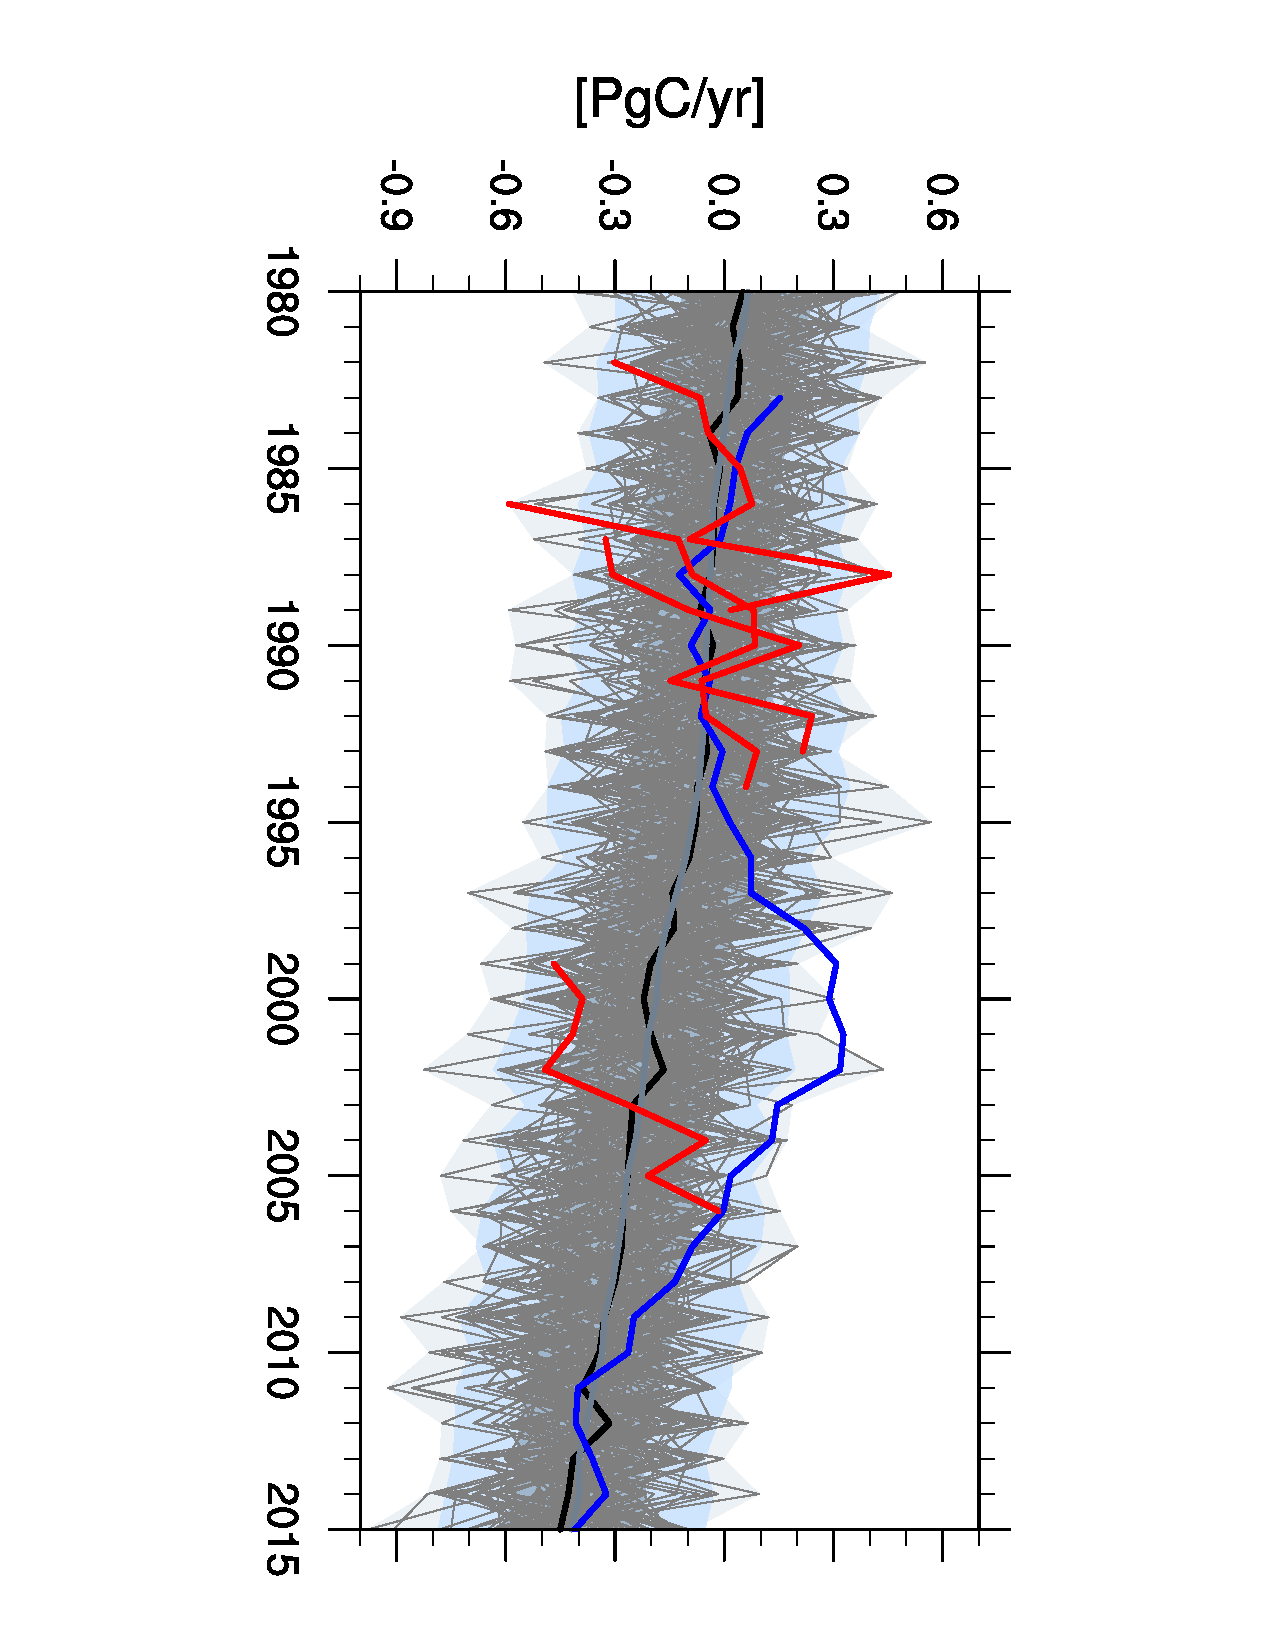
\includegraphics[scale=0.43,trim=4cm 0cm 4cm 0cm,clip,angle=90]{gfx/co2flux_SO_timeseries_ym_mar-feb_35S_1980_2015_trend_8}
       % \label{fig:example-b}%
        \caption{Evolution of the Southern Ocean carbon sink anomaly south of 35$^\circ$S. Grey lines show the 100 ensemble members, the black line the ensemble median, the gray shading is the range of the ensemble, the blue shading is the 2$\sigma$ ensemble spread, the red lines are decreasing sink trend candidates, the blue line is the SOM-FFN observation-based estimate \citep{landschuetzer2015}; negative values indicate anomalous uptake with respect to the 1980s}
        \label{fig:SOCS}
\end{figure}
